%
% File eacl2017.tex
%
%% Based on the style files for ACL-2016
%% Based on the style files for ACL-2015, with some improvements
%%  taken from the NAACL-2016 style
%% Based on the style files for ACL-2014, which were, in turn,
%% Based on the style files for ACL-2013, which were, in turn,
%% Based on the style files for ACL-2012, which were, in turn,
%% based on the style files for ACL-2011, which were, in turn,
%% based on the style files for ACL-2010, which were, in turn,
%% based on the style files for ACL-IJCNLP-2009, which were, in turn,
%% based on the style files for EACL-2009 and IJCNLP-2008...

%% Based on the style files for EACL 2006 by
%%e.agirre@ehu.es or Sergi.Balari@uab.es
%% and that of ACL 08 by Joakim Nivre and Noah Smith

\documentclass[11pt]{article}

\usepackage[a4paper]{geometry}
\usepackage{eacl2017}
\usepackage{times}
\usepackage{url}
\usepackage{latexsym}

% Added from MacDonald's .tex file ----------------------------
\usepackage{float}
\usepackage{caption}

% amsmath package, useful for mathematical formulas
\usepackage{amsmath}

% amssymb package, useful for mathematical symbols
\usepackage{amssymb}

% hyperref package, useful for hyperlinks
% \usepackage{hyperref}

% graphicx package, useful for including eps and pdf graphics
% include graphics with the command \includegraphics
\usepackage{graphicx}

% Sweave(-like)
\usepackage{fancyvrb}
\DefineVerbatimEnvironment{Sinput}{Verbatim}{fontshape=sl}
\DefineVerbatimEnvironment{Soutput}{Verbatim}{}
\DefineVerbatimEnvironment{Scode}{Verbatim}{fontshape=sl}
\newenvironment{Schunk}{}{}
\DefineVerbatimEnvironment{Code}{Verbatim}{}
\DefineVerbatimEnvironment{CodeInput}{Verbatim}{fontshape=sl}
\DefineVerbatimEnvironment{CodeOutput}{Verbatim}{}
\newenvironment{CodeChunk}{}{}

% -------------------------------------------------------------------------

% Added so that I could use the `fancy_lists` pandoc extension. If you don't want this or it's giving you errors, remove the line below and the line in `acl_article.R` that adds `+fancy_lists`
\def\tightlist{}


% If you have:
%   final_submission: yes
%   eaclpaperid: <your ID number>
% in the .Rmd metadata, it should have automatically
% added "\eaclfinalcopy" and "\def\eaclpaperid{<your ID number>}" above


% You can expand the titlebox if you need extra space
% to show all the authors. You can do this by uncommenting
% the line in the Rmd header:
%   # titlebox_length: "5cm"
% and substituting it with your own length.
% Please note that the minimum length is 5cm--they will
% check it and make you change it if it's smaller than that.

\newcommand\BibTeX{B{\sc ib}\TeX}

\title{How to Make a Camera-Ready Proceedings Contribution}


\author{{\large \bf Author 1} \\ \texttt{author1@university.edu} \\ Department of Psychology \\ Some University \And {\large \bf Author 2} \\ \texttt{author1@university.edu} \\ Department of Psychology \\ Some University}

\date{}

\begin{document}

\maketitle

\begin{abstract}
This document contains the instructions for preparing a camera-ready
manuscript for the proceedings of EACL-2017. The document itself
conforms to its own specifications, and is therefore an example of what
your manuscript should look like. These instructions should be used for
both papers submitted for review and for final versions of accepted
papers. Authors are asked to conform to all the directions reported in
this document.
\end{abstract}

\section{Methods}\label{methods}

\subsection{Nouns}\label{nouns}

We used data from Wordbank (Frank et al., 2017), an open repository
aggregating cross-linguistic language developmental data of the
MacArthur-Bates Communicative Development Inventory (CDI), a parent
report vocabulary checklist, Toddler version. Parent report is a
reliable and valid measure of children's vocabulary (Fenson et al.,
1994). We used a set of nouns representing hand-checked translation
equivalents across 10 languages (available in Wordbank database). We
``assume'' (i should ask what were the criteria for the unilemma
selection) that this set of translation equivalents is representative of
a core shared vocabulary across all children (in different cultures) by
around 30 months,

The conceptual organization derived from this shared vocabulary is
obviousely identical across languages, but we investigate whether there
are systematic cross-lingusitc variations in the order of aquisition of
words that make up this vocabulary, and crucially, whether such
variation influences the induced conceptual organization at different
points in time. In fact, differences in the order of acqusition of words
do not necessarily give rise to different conceptual organization.
Imagine that two languages vary in whether ``cow'' or ``dog'' is
acquired first. This difference will not change the induced conceptual
organization across time since both ``dog'' and ``cow'' are instances of
the same high-level concept ``animal''.

\begin{CodeChunk}
\captionsetup{width=0.8\textwidth}\begin{figure}[h]

{\centering 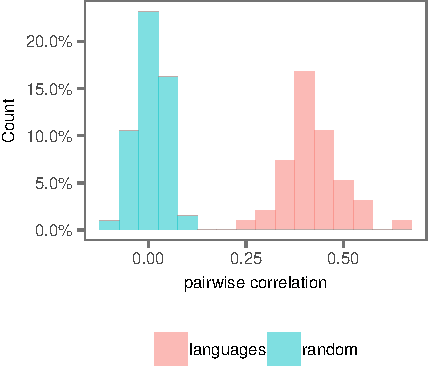
\includegraphics{figs/unnamed-chunk-1-1} 

}

\caption[bla bla]{bla bla}\label{fig:unnamed-chunk-1}
\end{figure}
\end{CodeChunk}

\subsection{Features}\label{features}

We used two sources of information which represent two ways words may be
related to one another in the semantic network. The first source was the
MacRae features (McRae et al., 2005). These features were collected by
giving adult participants a set of nouns and prompting them to provide
various kinds of properties (perceptual, functional, encyclopedic, and
taxonomic). We followed Hills et al. 2010 in excluding the encyclopedic
and taxonomic properties as their role may not be important at this
stage of development. The other source was the semantic similarity
derived based on co-occurrence in the corpus of CHILDES, using word2vec.

\subsection{Network}\label{network}

We constructed networks using CDI words as nodes. Pairs of words were
linked by an edge weighted by the number of shared MacRae feature or
with the continuous distance obtained via Word2vec. To model change in
the conceptual organization from month to month, we constructed a
different network at each month, based on the words that have been
acquired by that month. We defined the age of acquisiton of a given word
by the month at which this noun was produced by at least 50\% of
children, in each language (Goodman et al., 2008).

\subsection{Small World properties}\label{small-world-properties}

We test whether the networks display the so-called ``small-world''
properties similar to other semantic and real-world networks (Steyvers
\& Tenenbaum, 2005; Watts \& Strogatz, 1998). Small world properties are
characterized with the average clustering coefficient \(C\) and the
average shortest path \(L\). The former measures the extent to which the
network is clustered, i.e., made of highly connectned sub-networks,
whereas the latter measures the typical separation between tow nodes in
the network. A network is small-word if it has a higher clustering
coeffient comapred to a randomly connected network of the same size
\(C \gg C_{random}\), while still having a shorest path length as small
as the one typically observed in random networks, that is
\(L \approx L_{random}\).

\begin{CodeChunk}
\captionsetup{width=0.8\textwidth}\begin{figure*}[h]

{\centering 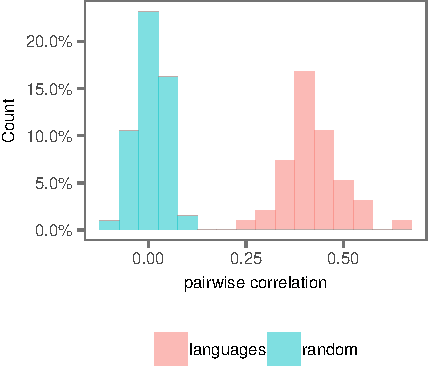
\includegraphics{figs/unnamed-chunk-2-1} 

}

\caption[bla bla]{bla bla}\label{fig:unnamed-chunk-2}
\end{figure*}
\end{CodeChunk}

\subsection{Clustering analysis}\label{clustering-analysis}

We identified network clusters using WalkTrap (Pons \& Latapy, 2006), a
community detection algorithm based on the fact that a random walker
tends to be trapped in dense parts of a network corresponding to highly
interconnected sub-groups of nodes.

\subsection{Evaluation of clusterings aross
development}\label{evaluation-of-clusterings-aross-development}

We note \(\mathcal{C}_t\) the clustering at month \(t\), based on the
subset of the vocabulary acquired by that month in each language. The
evaluation consists in comparing \(\mathcal{C}_t\) to the final
clustering \(\mathcal{C}^*\) obtained using the full vocabulary by the
last month of acquisition (i.e., \(\mathcal{C}^*\)=\(\mathcal{C}_t\) for
\(t\)=30 months). Such comparison allows us to study how words acquired
at different points in time may induce changes in the conceptual
organization. In addition, we investigate consistency and variability in
this change across languages.

We compare \(\mathcal{C}_t\) to \(\mathcal{C}^*\) using a standard
method in clustering comparison, which is based on counting word pairs
on which the two clusterings agree or disagree (Rand, 1971; Hubert and
Arabie, 1985). A pair of words learned by month \(t\) can fall under one
of the four follwoing cases: 1) pairs that are placed in the same
cluster under \(\mathcal{C}_t\) and in the same cluster under
\(\mathcal{C}^*\) (True positives, noted as \(tp(\mathcal{C}_t)\)), 2)
pairs placed in different clsuters under \(\mathcal{C}_t\) and in
different clusters under \(\mathcal{C}^*\) (True negatives,
\(tn(\mathcal{C}_t)\)), 3) pairs placed in the same cluster under
\(\mathcal{C}_t\) and in different clusters under \(\mathcal{C}^*\)
(False positive, \(fp(\mathcal{C}_t)\)), and 4) pairs placed in
different clusters under \(\mathcal{C}_t\) and in the same cluster under
\(\mathcal{C}^*\) (False negatives, \(fn(\mathcal{C}_t)\)).

The clustering precison \(P(\mathcal{C}_t)\) and recall
\(R(\mathcal{C}_t)\) are defiend as follows:

\[
P(\mathcal{C}_t) = \frac{|tp(\mathcal{C}_t)|}{|tp(\mathcal{C}_t)| + |fp(\mathcal{C}_t)|}
\] \[
R(\mathcal{C}_t) = \frac{|tp(\mathcal{C}_t)|}{|tp(\mathcal{C}_t)| + |fn(\mathcal{C}_t)|}
\] Both Precison and Recall converge to 1 (perfect score) as
\(\mathcal{C}_t\) becomes more and more similar to \(\mathcal{C}^*\). If
precision starts low before converging to 1 (as opposed to being a
constant at 1), this pattern would indicate that some pairs that should
be differentiated are initially lumped together, suggesting a process of
``differentiation'' over development. Similarly, if we observe an
increase in Recall, this pattern would indicate that some pairs that
should be associated are initially differentiate, suggesting a process
of ``coelescence'' over development.

\subsection{Word ordering}\label{word-ordering}

The question we are addressing is whether the order of acqusition of
words affect the

\section{Results}\label{results}

For real and random: results show that both precision and recall
increase across development, suggesting that the conceptual organization
undergoes both differentiation for some word pairs (example), and
coelescecne for other pairs (examples).

For within-cluster: precision is high, but recall is low: explain why

How to explain this change?

\begin{quote}
Assuming a random/real ranking of words: -Some words may be lamped
together initially (even if we force a relatively high number of
clusters) because of the smaller vocabulary size? Can we have an example
of this? Are the other clsuters empty? -Some words may be differentiated
initially because of the forcing? -Is there a roleof noise? maybe
clustering is just more random for smaller size vocabulary?
\end{quote}

\begin{quote}
Assuming a with-cluster ranking of words: -Some words may be lamped
together initially (even if we force a relatively high number of
clusters): this does not happen, at least while we are still working
with the first cluster\ldots{}that's why precision is generally high
-Some words may be differentiated initially because they
\end{quote}

\subsection{Order of word learning}\label{order-of-word-learning}

\section{Sudy of the conceptual
development}\label{sudy-of-the-conceptual-development}

Models

\section{Important citation stuff!
READ!}\label{important-citation-stuff-read}

\subsection{Why we can't have nice
things}\label{why-we-cant-have-nice-things}

So because the ACL committee wants their \texttt{.tex} files all nice
and consistent, the old version of this package isn't good for what they
want. The Markdown-to-Latex conversion would automatically add in the
references and citations, but would literally hardcode them into the
\texttt{.tex} file. We can't have that, now can we? The only ways you
were allowed to cite in your \texttt{.tex} file was with
\texttt{\textbackslash{}cite\{Gusfield97\}},
\texttt{\textbackslash{}shortcite\{Gusfield97\}}, or
\texttt{\textbackslash{}newcite\{Gusfield97\}}, which corresponded to
``(Gusfield, 1997)'', ``(1997)'', or ``Gusfield (1997)'', respectively.

This means you couldn't do anything like ``(e.g., Gusfield, 2017)'', and
their \texttt{.bst} file was incompatible with \texttt{natbib}.
Obviously. However, I have come to the rescue. In the
\texttt{eacl2017.sty} file in this package, I have added my own bit of
magic: the \texttt{\textbackslash{}barecite\{\}} command, which
corresponds to ``Burchill, 2017''. Notice this version doesn't have
parentheses, so you can get stuff like ``(e.g., Burchill, 2017)'' with
\texttt{(e.g.,\ \textbackslash{}barecite\{Gusfield97\})}. Just be
careful about making sure you don't forget parentheses. Also not that
when you submit the \texttt{.zip} folder, you should make sure to
include the edited \texttt{eacl2017.sty} file.

\subsection{Examples}\label{examples}

\begin{itemize}
\tightlist
\item
  \texttt{\textbackslash{}cite\{Gusfield97\}} becomes \cite{Gusfield97}
\item
  \texttt{\textbackslash{}shortcite\{Gusfield97\}} becomes
  \shortcite{Gusfield97}
\item
  \texttt{\textbackslash{}newcite\{Gusfield97\}} becomes
  \newcite{Gusfield97}
\item
  \texttt{\textbackslash{}barecite\{Gusfield97\}} becomes
  \barecite{Gusfield97}
\item
  \texttt{\textbackslash{}cite\{Gusfield97,Aho72\}} becomes
  \cite{Gusfield97,Aho72}
\item
  \texttt{\textbackslash{}barecite\{Gusfield97,Aho72\}} becomes
  \barecite{Gusfield97,Aho72}
\end{itemize}

\textbf{Wait, \emph{are those citations appearing as question marks?}
Don't worry, read on!}

\subsection{The two-step process of knitting this
file}\label{the-two-step-process-of-knitting-this-file}

Because the ACL's you-need-to-use-our-citing-function formatting doesn't
work well with R Markdown--which really likes to compile its own
citations--knitting this is now a two-step process. After you get it how
you want it in RMarkdown, knit as usual. You'll see that all citations
are question marks, and that the bibliography is missing. This is
natural, don't panic.

For the current purposes, let's assume this file we're in right now is
called \texttt{acl\_draft.Rmd}. Navigate into the directory containing
\texttt{acl\_draft.Rmd} via a terminal. Then run the following command
(swapping out your actual file name for ``acl\_draft'')

\texttt{pdflatex\ acl\_draft.tex;\ pdflatex\ acl\_draft.tex;\ bibtex\ acl\_draft.aux;\ pdflatex\ acl\_draft.tex;\ pdflatex\ acl\_draft.tex}

Now, check the \texttt{.pdf} file. If all went well, it should now have
all the citations in it as well as the reference section. Good luck!

\section{General Formatting
Instructions}\label{general-formatting-instructions}

All the default content below is lifted directly from Kyle MacDonald's
Cogsci 2016 project (\url{https://github.com/kemacdonald/cogsci2016}),
which this entire package is based on. I haven't changed it, so it's up
to you to ignore as you please.

For general information about authoring in markdown, see
**\url{http://rmarkdown.rstudio.com/authoring_basics.html.**}

For standard spoken papers and standard posters, the entire contribution
(including figures, references, everything) can be no longer than six
pages. For abstract posters, the entire contribution can be no longer
than one page. For symposia, the entire contribution can be no longer
than two pages.

The text of the paper should be formatted in two columns with an overall
width of 7 inches (17.8 cm) and length of 9.25 inches (23.5 cm), with
0.25 inches between the columns. Leave two line spaces between the last
author listed and the text of the paper. The left margin should be 0.75
inches and the top margin should be 1 inch.
\textbf{The right and bottom margins will depend on whether you use
U.S. letter or A4 paper, so you must be sure to measure the width of
the printed text.} Use 10 point Times Roman with 12 point vertical
spacing, unless otherwise specified.

The title should be in 14 point, bold, and centered. The title should be
formatted with initial caps (the first letter of content words
capitalized and the rest lower case). Each author's name should appear
on a separate line, 11 point bold, and centered, with the author's email
address in parentheses. Under each author's name list the author's
affiliation and postal address in ordinary 10 point type.

Indent the first line of each paragraph by 1/8\textasciitilde{}inch
(except for the first paragraph of a new section). Do not add extra
vertical space between paragraphs.

\section{First-Level Headings}\label{first-level-headings}

First level headings should be in 12 point , initial caps, bold and
centered. Leave one line space above the heading and
1/4\textasciitilde{}line space below the heading.

\subsection{Second-Level Headings}\label{second-level-headings}

Second level headings should be 11 point , initial caps, bold, and flush
left. Leave one line space above the heading and 1/4\textasciitilde{}
line space below the heading.

\subsubsection{Third-Level Headings}\label{third-level-headings}

Third-level headings should be 10 point , initial caps, bold, and flush
left. Leave one line space above the heading, but no space after the
heading.

\section{Formalities, Footnotes, and
Floats}\label{formalities-footnotes-and-floats}

\subsection{Footnotes}\label{footnotes}

Indicate footnotes with a number\footnote{Sample of the first
footnote.} in the text. Place the footnotes in 9 point type at the
bottom of the page on which they appear. Precede the footnote with a
horizontal rule.\footnote{Sample of the second footnote.}

\subsection{Figures}\label{figures}

All artwork must be very dark for purposes of reproduction and should
not be hand drawn. Number figures sequentially, placing the figure
number and caption, in 10 point, after the figure with one line space
above the caption and one line space below it. If necessary, leave extra
white space at the bottom of the page to avoid splitting the figure and
figure caption. You may float figures to the top or bottom of a column,
or set wide figures across both columns.

\subsection{Two-column images}\label{two-column-images}

You can read local images using png package for example and plot it like
a regular plot using grid.raster from the grid package. With this method
you have full control of the size of your image. \textbf{Note: Image
must be in .png file format for the readPNG function to work.}

You might want to display a wide figure across both columns. To do this,
you can change the \texttt{fig.env} chunk option to \texttt{figure*}. To
align the image in the center of the page, set \texttt{fig.align} option
to \texttt{center}.

\begin{CodeChunk}
\begin{figure*}[h]

{\centering 
\includegraphics{figs/2-col-image-1} 

}

\caption[This image spans both columns]{This image spans both columns.}\label{fig:2-col-image}
\end{figure*}
\end{CodeChunk}

\subsection{One-column images}\label{one-column-images}

Single column is the default option, but if you want set it explicitly,
set \texttt{fig.env} to \texttt{figure}.

\begin{CodeChunk}
\begin{figure}[H]

{\centering 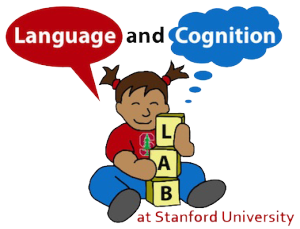
\includegraphics{figs/image-1} 

}

\caption[One column image]{One column image.}\label{fig:image}
\end{figure}
\end{CodeChunk}

\subsection{R Plots}\label{r-plots}

You can use R chunks directly to plot graphs. And you can use latex
floats in the fig.pos chunk option to have more control over the
location of your plot on the page. For more information on latex
placement specifiers see
**\url{https://en.wikibooks.org/wiki/LaTeX/Floats,_Figures_and_Captions**}

\begin{CodeChunk}
\begin{figure}[H]

{\centering 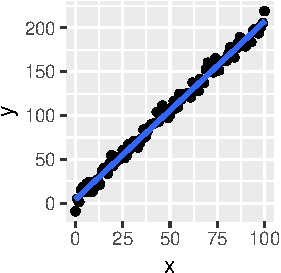
\includegraphics{figs/plot-1} 

}

\caption[R plot]{R plot}\label{fig:plot}
\end{figure}
\end{CodeChunk}

\subsection{Tables}\label{tables}

Number tables consecutively; place the table number and title (in 10
point) above the table with one line space above the caption and one
line space below it, as in Table 1. You may float tables to the top or
bottom of a column, set wide tables across both columns.

You can use the xtable function in the xtable package.

\begin{table}[H]
\centering
\begin{tabular}{rrrrr}
  \hline
 & Estimate & Std. Error & t value & Pr($>$$|$t$|$) \\ 
  \hline
(Intercept) & 0.07 & 0.09 & 0.7 & 0.49 \\ 
  x & 1.92 & 0.09 & 20.4 & 0.00 \\ 
   \hline
\end{tabular}
\caption{This table prints across one column.} 
\end{table}

\section{Acknowledgements}\label{acknowledgements}

Place acknowledgments (including funding information) in a section at
the end of the paper.

\bibliography{eacl2017}
\bibliographystyle{eacl2017}

\end{document}

